\documentclass[12pt,a4paper]{article}
\usepackage{lipsum}
\usepackage[T1]{fontenc}
\usepackage{amsmath}
\usepackage{hyperref}
\usepackage{amssymb}
\usepackage{graphicx}
\usepackage{geometry}
\usepackage[table]{xcolor}
\usepackage{array}
\usepackage{newtxtext,newtxmath}
\usepackage{sectsty}
\usepackage{titlesec}
\usepackage[none]{hyphenat}
\newgeometry{
    top=1in,
    bottom=1in,
    left=1.5in,
    right=1in
}
\hypersetup{
    colorlinks,
    citecolor=black,
    filecolor=black,
    linkcolor=black,
    urlcolor=black
}

\titlelabel{\thetitle.\quad}

% center section text
% \sectionfont{ \centering}

\renewcommand{\baselinestretch}{1.5}
\title{Comparison of different Image Super Resolution Techniques}
\author{Kabin Poudel}
\begin{document}
\pagenumbering{roman}
% \addcontentsline{toc}{section}{COVER PAGE}
\thispagestyle{empty} % This will hide pagenumber in title page


% Title page (Design in your own way)

{
	\thispagestyle{empty}
	\centering
	\normalsize
	  
	\includegraphics[width=1.3in]{./figures/TUlogo.png}\\[0.5cm]
	{\bf{TRIBHUVAN UNIVERSITY}\\
	{INSTITUTE OF ENGINEERING}\\
	PURWANCHAL CAMPUS}
	\\[1cm]
	
	{\bf COMPARISON OF DIFFERENT IMAGE SUPER RESOLUTION TECHNIQUES}\\[1cm]
	
	BY:\\
	{\bf ABHINAV JAISHI \hspace{1in} (44002)}\\
	{\bf MEGHA THAKUR    \hspace{1in} (44021)}\\
	{\bf SANGHARSHA DAHAL \hspace{0.6in} (44029)}\\
	{\bf KABIN POUDEL     \hspace{1in}\space\space\space\space (44047)}\\[1.5cm]

	
% 	A PROJECT WAS SUBMITTED TO THE DEPARTMENT OF ELECTRONICS AND COMPUTER
% 	ENGINEERING IN PARTIAL FULFILLMENT OF THE REQUIREMENT FOR THE BACHELOR'S
% 	DEGREE IN Electronics and Communication ENGINEERING\\[1.5cm]



	A FINAL REPORT TO THE DEPARTMENT OF ELECTRONICS AND COMPUTER
	ENGINEERING IN PARTIAL FULFILLMENT OF THE REQUIREMENT FOR THE BACHELOR'S
	DEGREE IN ELECTRONICS, COMMUNICATION AND INFORMATION ENGINEERING\\[0.5cm]
	% ~
	
	{\bf DEPARTMENT OF ELECTRONICS AND COMPUTER ENGINEERING\\
	PURWANCHAL CAMPUS\\
	DHARAN, NEPAL}\\[1.5cm]

	{\bf\today}
	
	
}

%%% Local Variables:
%%% mode: plain-tex
%%% TeX-master: t
%%% End:
\newpage
% \addcontentsline{toc}{section}{TITLE PAGE}
\thispagestyle{empty}
\begin{titlepage}
    \centering
{\fontsize{12pt}{14pt}\bfseries\textcolor{black}{COMPARISON OF DIFFERENT IMAGE SUPER RESOLUTION TECHNIQUES}\par}
\vspace{2.0cm}
       {BY:} \par {ABHINAV JAISHI}({PUR076BEI001})
            \par {MEGHA THAKUR}({PUR076BEI021})
            \par {SANGHARSHA DAHAL}({PUR076BEI029})
            \par {KABIN POUDEL}({PUR076BEI047})
       \vspace{2.0cm}\par
    Project Supervisor\par
    Asst. Prof. Pukar Karki\par
    \vspace{2.0cm}
    {A project submitted to the Department of Electronics and Computer Engineering in partial fulfillment of the requirements for the Bachelor’s Degree in Electronics, Communication and Information Engineering}\par
        \vspace{2.0cm}\par

    {Department of Electronics and Computer Engineering\\ Purwanchal Campus, Institute of Engineering \\ Tribhuvan University\\ Dharan, Nepal}\par
        \vspace{2.0cm}\par
        
        \today
\end{titlepage}
\newpage
\addcontentsline{toc}{section}{COPYRIGHT}
\section*{\copyright COPYRIGHT}
\par
The author has agreed that the Library, Department of Electronics and Computer Engineering, Purwanchal Campus, Institute of Engineering may make this report freely
available for inspection. Moreover, the author has agreed that permission for extensive
copying of this project report for scholarly purpose may be granted by the supervisor(s)
who supervised the thesis work recorded herein or, in their absence, by the Head of
the Department wherein the thesis report was done. It is understood that the
recognition will be given to the author of this report and to the Department of
Electronics and Computer Engineering, Purwanchal Campus, Institute of Engineering in
any use of the material of this thesis report. Copying or publication or the other use of
this report for financial gain without approval of the Department of Electronics and
Computer Engineering, Purwanchal Campus, Institute of Engineering and author’s
written permission is prohibited.\\
\\
Request for permission to copy or to make any other use of the material in this report
in whole or in part should be addressed to:\\
\\
Head\\
Department of Electronics and Computer Engineering\\
Purwanchal Campus, Institute of Engineering\\
Dharan , Sunsari\\
Nepal
\newpage
\addcontentsline{toc}{section}{DECLARATION}
\section*{DECLARATION}
We declare that the work hereby submitted for Bachelors of Engineering in Electronics, Communication and Information at Institute of Engineering, Purwanchal Campus entitled \textbf{`` COMPARISON OF DIFFERENT IMAGE SUPER RESOLUTION TECHNIQUES"} is our own work and has not been previously submitted by me at any university for any academic award.\\
We authorize Institute of Engineering, Purwanchal Campus to lend this report to other institution or individuals for the purpose of scholarly research.
\vspace{1cm}\\
ABHINAV JAISHI (44002)\\
MEGHA THAKUR (44021)\\
SANGHARSHA DAHAL (44029)\\
KABIN POUDEL (44047)\\
\\
\today
\newpage
\addcontentsline{toc}{section}{RECOMMENDATION}
\section*{RECOMMENDATION}

\newpage

\section*{ACKNOWLEDGEMENT}
\addcontentsline{toc}{section}{ACKNOWLEDGEMENT}

We would like to take this opportunity to express our deepest gratitude and sincerest appreciation to all those who gave helped us to complete our project. We would like to give our special thanks to our project supervisor { \bf Asst. Prof. Pukar Karki} whose help, suggestions, invaluable guidance and motivating feedback made the completion of the project a reality.\\
\\
We would also like to thank {\bf Asst. Prof. Pravin Sangroula}, Head of Department of Electronics and Computer Engineering for their regular support and co-operation. We would also like to acknowledge the help and co-operation of all the teaching and non-teaching staffs of the campus for the attainment of the project.\\
\\
Lastly, we would like to express our deep appreciation and gratitude to our family, friends and well-wishers who have always helped us to keep up the morale and excitement in our work; without their encouragement and love we would not have achieved
our goals.
\vspace{1cm}\\
ABHINAV JAISHI (PUR076BEI001)\\
MEGHA THAKUR (PUR076BEI021)\\
SANGHARSHA DAHAL (PUR076BEI029)\\
KABIN POUDEL (PUR076BEI047)\\
\\

\newpage

\section*{ABSTRACT}
\addcontentsline{toc}{section}{ABSTRACT}

Image Super Resolution (ISR) techniques have been developed for a long time. It have witnessed substantial advancements in recent years, aiming to enhance the visual quality of low-resolution images. This study compares different ISR technique based on deep learning and suggest which works best on different scenarios.


This paper includes comparison of SISR techniques including SRGAN, SRResNet and SRCNN. Each technique has distinct architectural approaches and training methodologies, addressing the common goal of reconstructing high-resolution images from their low-resolution counterparts. The study aims to provide valuable insights for enthusiasts and researcher interested in using SISR techniques for high-quality image super-resolution. Each of these techniques has its strengths and weaknesses, and understanding them can help researchers and enthusiasts choose the most suitable method for their specific needs.
\\
\\
\textit {{\bf Keywords:}  Super Resolution Generative Adversarial Network (SRGAN), Super Resolution Residual Network (SRResNet), Super Resolution Convolutional Neural Network (SRCNN), Single Image Super Resolution (SISR) }
\newpage
{
  \setlength{\parskip}{0em}
  \renewcommand\contentsname{TABLE OF CONTENTS} % This will change heading text
  \tableofcontents \addcontentsline{toc}{section}{TABLE OF CONTENTS}
}

% List of figures - if any

\newpage
\listoffigures 
\addcontentsline{toc}{section}{LIST OF FIGURES}

% List of tables- if any

\newpage
\listoftables 
\addcontentsline{toc}{section}{LIST OF TABLES}




\newpage
\pagenumbering{arabic}
\section{INTRODUCTION}
Image super resolution is a technique used to enhance the resolution and quality of
image beyond its original size. It is useful technique in the field of image processing. It
can be used to enhance the quality of image captured in night, shaky image etc. There
are various techniques and algorithm used for image super resolution, including both
traditional methods and deep learning-based approaches. Traditional super image
resolution techniques are based on mathematics techniques. These techniques have
been used for many years. Some of the traditional super resolution techniques include:
Interpolation, Edge-Directed interpolation, Bayesian methods etc. Traditional methods
have certain limitations compared to deep learning approaches. They may struggle to
capture complex patterns and textures, and their performance is often constrained by
the hand-crafted features and assumptions used in the algorithms.
Deep learning based super resolution typically employs Convolution Neural
Network (CNN) to learn the mapping between low-resolution and high-resolution
images. The network is trained on large dataset of paired low-resolution and high-
resolution images. During training, the networks learn to identify patterns and features
that enables it to generate high-resolution details from low-resolution inputs.

% \clearpage

\subsection{Statement of problem}
The need of super image resolution arises when we encounter low-resolution images
that lack the desired level of detail and clarity that may be due to various factors such as limitations in capturing hardware, resizing
operations, or compression from social media. There is not only need of Super Resolution, We also need to know which method works best for which usecase.
% add some lines of  content and remove newpage  below

\subsection{Objectives} 
% spandan
\begin{itemize}
    \item To implement different Super Resolution Algorithms.
    \item To compare them to findout their best usecases.
\end{itemize}

\subsection{Scope and Applications}
Image super resolution has numerous practical applications in field
like photography, surveillance, and digital art where enhanced image quality is crucial
for accurate decision-making, analysis, and interpretation. The development of efficient
and accurate super-resolution method involves exploring traditional signal processing
techniques, as well as cutting-edge deep learning approaches, to achieve optimal results
while considering computational efficiency and resource constraints. We can understand that not every technique will work well in every scenarios. So, There is a need for understanding the techniques to use them where they perform best.\\
Super image resolution can be used for following things: 
\begin{enumerate}
    \item Super resolution can be used to improve the resolution of old and degraded
    images, preserving historical photographs, artworks, and documents. 
    \item Super resolution can be used in digital cameras and smartphones to provide
    better zoom capabilities without significant loss of image quality.
    \item Super resolution can enhance the resolution of individual frames in videos,
    leading to improved video quality and better extraction of information. 
    \item In surveillance systems, low resolution camera feeds can be upscaled to improve
    the ability to identify faces, license plates, or other critical details, helping in
    investigations. 
    
\end{enumerate}

\newpage
\section{LITERATURE REVIEW}
In the timeline of image scaling process, the first used methods were different interpolation techniques and sparse representation-based methods. But with the advent
of deep-learning based image scaling techniques interpolation methods were less commonly used in image enhancement.

D. Han (2013) {\bf“Comparison of commonly used image interpolation methods”} discusses multiple interpolation methods like nearest neighbor, bilinear, bicubic, etc. Although interpolation is fast but have some disadvantages. But using these methods was not optimal for our use case as they may lead to the loss of fine details and sharpness in image and can amplify noise present in image which may not be accurate in real-world images.\cite{r1}

C. Dong, et. al, {\bf“Image super-resolution using deep convolutional networks”} is a seminal paper on use of Deep Learning for the use of for the task of SR. It only consists of three layers and requires the LR image to be up-sampled using bicubic interpolation prior to being processed by the network, but it was shown to outperform the state-ofthe-art methods of that time.\cite{r2}

C. Ledig et al., {\bf“Photo-realistic single image super-resolution using a generative adversarial network”} discusses about a Generative Adversarial Network (GAN) for image super-resolution (SR). It is the first framework capable of inferring photo-realistic natural images for 4x upscaling factors using GAN. To achieve this, it uses
a perceptual loss function which consists of an adversarial loss and a content loss. The adversarial loss pushes the solution to the natural image manifold using a discriminator
network that is trained to differentiate between the super-resolved images and original photo-realistic images. In addition, it uses a content loss motivated by perceptual
similarity in VGG space instead of similarity in pixel RGB space. This deep residual network is able to recover photo-realistic textures from heavily down sampled images on public
benchmarks. An extensive mean-opinion-score (MOS) test shows hugely significant gains in perceptual quality using SRGAN. The MOS scores obtained with SRGAN are
closer to those of the original high-resolution images than to those obtained with any state-of-the-art method at the time. Both SRResNet and SRGAN are explained in related theory portion of the study.\cite{r3}

\newpage
\section{HARDWARE AND SOFTWARE REQUIREMENTS}
\subsection{Hardware Requirements}
We used the system with following specifications for training:
\begin{itemize}
    \item PC with Windows 11
    \item 16 GB RAM 
    \item Nvidia Geforce GTX 1050(4GB)
    \item 256 GB storage
    \item Processor: Intel(R) Core(TM) i5-8300H CPU @ 2.30GHz
\end{itemize}
\subsection{Software Requirements}
The software requirements for developing, training, evaluating, and deploying the
model effectively are listed below: 
\begin{enumerate}
    \item {\bf Integrated Development Environment (IDE):} We used Visual Studio Code (VS Code) as IDE for training, testing and documentation. 
    It  is a popular feature rich code editor. It is available on Windows, macOS, and Linux.
    \item {\bf Version Control System:} We used Git and Github. Git is a distributed version control system. It allows multiple developers to collaborate on projects, keeping track of modifications, managing different versions of files, and merging changes.
    \item {\bf Web framework:} We simply used Streamlit framework. Streamlit is an open-source Python library that makes it remarkably easy to create and share beautiful, custom web apps for machine learning and data science.
    \item {\bf Deep-Learning Frameworks:} We used PyTorch. It is an open-source, Python-based deep learning library. It allows to build and train neural networks for various tasks like computer vision, natural language processing, and more.
\end{enumerate}
\newpage
\section{RELATED THEORY}
\subsection{Architectural Explanations}
Image Super Resolution upscales a Low-Resolution Image to High Resolution Image, filling in the missing pixels with the different techniques. There are other simpler methods to upscale images like Linear or Bi-cubic interpolation, but they do not generate any new information based on the environment and hence are not super useful to upscale an LR image. Deep Learning based methods require huge amounts of data so that the model is not overfitted, the dataset needs to contain an HR and LR version of the same image that are perfectly aligned to each other. We need to synthetically create LR images from HR images.\\
SR aims to then reverse whichever degradation process is considered, to retrieve the original underlying high-fidelity image. We have implemented SRCNN, SSResNet and SRGAN. Their architecture is explained below: 
\begin{enumerate}
    \item {\bf SRCNN:} Super-Resolution Convolutional Neural Network, is a deep learning architecture devised for single-image super-resolution tasks. Developed by {\bf Dong et al. in 2014} \cite{r2}, SRCNN revolutionized image enhancement by learning complex mappings between low-resolution and high-resolution images directly from data. Its architecture consists of multiple layers of convolutional neural networks (CNNs), which process input images in a hierarchical manner, gradually extracting high-level features. The architecture of SRCNN is given below:
    \begin{figure}[ht]
        \centering
        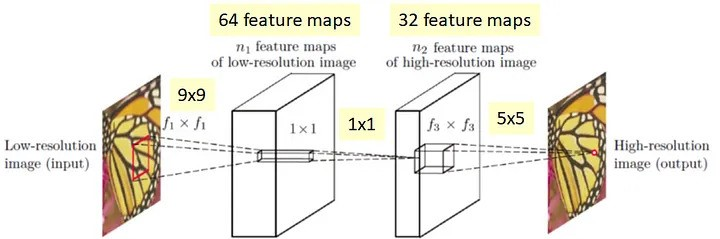
\includegraphics[width=5in]{./figures/srcnn.jpg}
        \caption{SRCNN Architecture}
    \end{figure} \\
    We converted image from training database into Y,Cb,Cr format and used only Y (Luminance) component for training the model. The primary loss function used in SRCNN is Mean Squared Error (MSE). We used Adam optimizer, optimizer is responsible for updating the network's parameters during the training process in order to minimize the chosen loss function.

    \item {\bf SRResNet:} The SRResNet is a fully convolutional network designed for 4x super-resolution. It incorporates residual blocks with skip connections to increase the optimizability of the network despite its significant depth. The SRResNet is trained and used as a standalone network and provides a nice baseline for the SRGAN – for both comparison and initialization. We use the following architecture for this network. 
    \begin{figure}[ht]
        \centering
        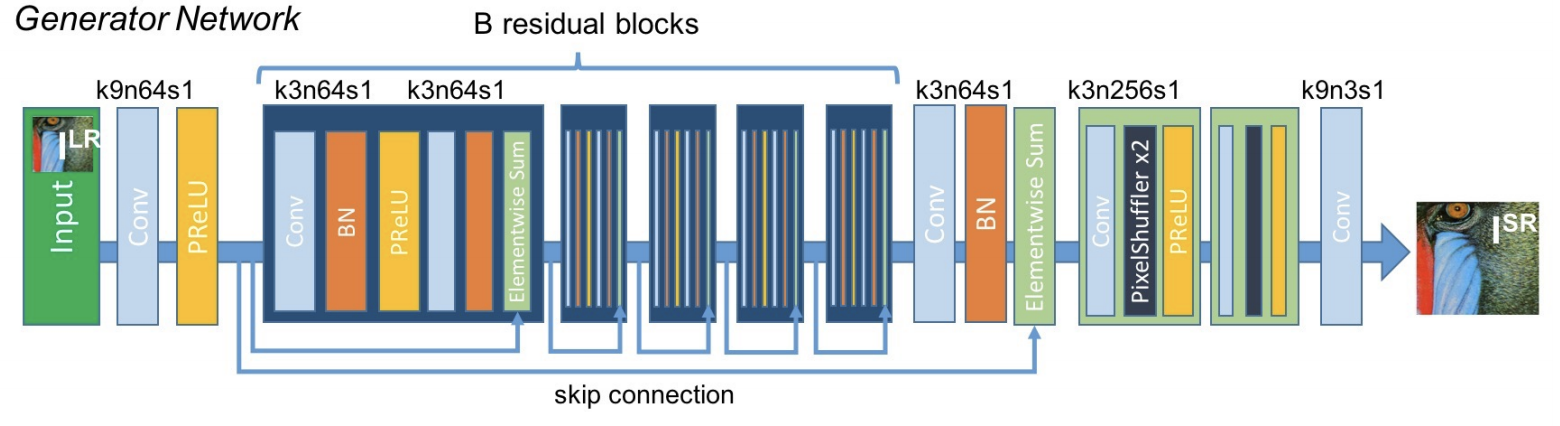
\includegraphics[width=6in]{./figures/generator.png}
        \caption{SRResNet Architecture or Generator of SRGAN}
    \end{figure} \\
    The SRResNet first contains convolution block of large Kernel Size 9x9, stride of 1 and 64 channels with PreLU activation. There are 16 residual blocks with convolution layer of Kernel size 3x3 followed by batch normalization, PreLU same conv layer again and batch normalization again. The output then is passed through same 3x3 conv layer and batch normalized. Two subpixel convolution blocks are used followed by PreLU activation each of which provides two times upscaling. Finally, a convolution with large kernel size of 9x9 and 1 stride with 3 out channels for RGB is done with Tanh activation to get super resolved image.\\ In Forward Pass, SRResNet produces a 4x upscaled image from provided low-res image using the above architecture. Mean-Squared Error (MSE) is used as the loss function to compare the upscaled image and original high-quality image. MSE is a type of content loss but here it only looks in RGB space of predicted and target images. Minimizing the MSE by changing the parameters of the network will make the model produce images closer to the original images.
    
    \item {\bf SRGAN:} Super-Resolution Generative Adversarial Network consist of two adversary networks Generator and Discriminator which are trained in tandem. The goal of the Generator is to learn to super-sample an image such that Discriminator can’t tell difference between artificial and natural origins. The interplay between these two networks leads to the improvement of both over time. \\
    The Generator learns not only by minimizing content loss, as in the case of the SRResNet but also by spying on the Discriminator's methods. By providing the Generator access to the Discriminator's inner workings in the form of the gradients produced therein when backpropagating from its outputs, the Generator can adjust its parameters in a way that alters the Discriminator's outputs in its favour. As the Generator produces more realistic high-resolution images, we use these to train the Discriminator, improving its discriminating abilities.
    \begin{figure}[ht]
        \centering
        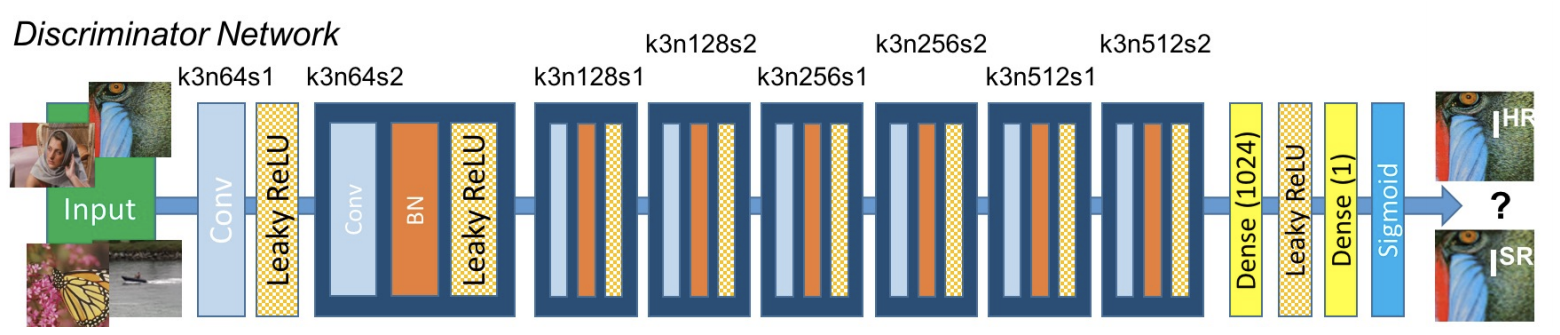
\includegraphics[width=6in]{./figures/discriminator.png}
        \caption{Discriminator Architecture}
    \end{figure} \\
    The Generator has same architecture as SRResNet. Training Discriminator is not different from any binary image classifier. It is trained on both real images and generated images from generator. In Forward Pass, it outputs the probability score $P_{HR}$. If the provided image was real, we desire the $P_{HR}$ to be as high as possible towards 1. And for generated image as low as possible towards 0. We use Binary Cross Entropy loss $-logP_{HR}$ when input image is real and $-logP_{SR}$ when image is generated. Here $P_{SR}=1-P_{HR}$. Minimizing these losses by changing the parameters will make discriminator predict higher probability for real images and lower probability for generated images.\\
    We use better content loss than that of SRResNet. In ResNet we use MSE loss in RGB space which produces overly smooth images with no finer details. There are a lot of possibilities of similar pixel combination that can be formed from low resolution image patch. When we use content loss in RGB space, it averages the output rather than choosing one of the combinations which would produce better result as an overly smooth “averaged” prediction will always have lower MSE.\\
    We can use CNN trained to classify images to find deeper meaning of patterns in images. This new representation space is more suitable for calculating content loss and can hallucinate new details showing creativity. We specifically use the VGG19 network as recommended in the paper. We use MSE-based content loss in this VGG space to compare the images. The use of content loss is only one component of the generator update, we use adversarial loss obviously. The super-resolved image is passed through the Discriminator with its weight frozen not to update the discriminator but to get the probability score $P_{HR}$ with misleading label and use the BCE loss $-logP_{HR}$ and resulting gradient information to update the Generator’s weights such that it produces images closer to its natural origin.
    GAN is trained in an interleaved fashion, where the generator and discriminator are alternatively trained for short periods of time just once before making the switch in this case.
\end{enumerate}
    \subsection{General Explanations}
    \begin{enumerate}
        \item {\bf Conv2d:} Conv2D stands for two-dimensional convolution, a fundamental operation in convolutional neural networks (CNNs). A convolutional layer applies a series of filters or kernels to an input image. Each filter detects specific patterns or features, like edges, textures, or shapes. The convolution operation involves sliding these filters over the input image, performing element-wise multiplication between the filter and the overlapping portions of the image, and then summing up the results to create a feature map.
        \begin{figure}[ht]
            \centering
            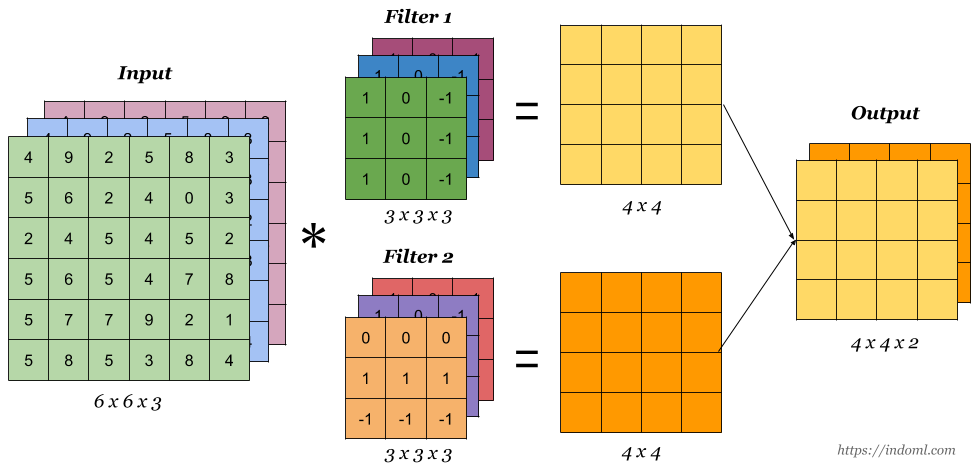
\includegraphics[width=5in]{./figures/conv2d.png}
            \caption{A visual explanation of convolution. }
        \end{figure} \\
        \begin{itemize}
            \item {\bf Kernel:} A kernel describes a filter that we are going to pass over an input image. The kernel will move over the whole image, from left to right, from top to bottom by applying a convolutional product. The output of this operation is called a filtered image.
            \item {\bf Stride:} Stride refers to the number of steps the convolutional filter moves horizontally or vertically during convolutional operation. For example, a stride of 2 means the filter moves two pixels at a time.
            \item {\bf Padding:} Padding describes the number of pixels added to the sides of the input channels before their convolutional filtering. Usually padding pixels are set to zero. This is particularly useful when we want the size of the output channels to be equal to the size of the input channels. When the kernel size is  3*3  then the output channel size is decreased by one on each size. To overcome this problem, we can use padding of 1.
            \item {\bf In channel:} In channel are used to describe how many channels are present in the input. For instance, if the input is an RGB image, then it has three channels. When using a Conv2d layer, we can specify the number of in channel, and the convolution operation is performed independently on each channel of the input. This allows the network to learn different features from different input channels, enabling it to detect various patterns within each channel.
            \item {\bf Out Channel:} Out Channel specifies the number of output channels produced by the convolutional layer. Each output channel corresponds to a distinct convolutional filter (or kernel) applied to the input.
        \end{itemize}
        \item {\bf Batch Normalization:} Batch normalization is a technique that normalizes the inputs to each layer in a network by adjusting and scaling to have zero mean and unit variance. This helps to reduce “internal covariate shift” problem which can hinder training. An internal covariant shift occurs when there is a change in input distribution to the network. When the input distribution changes, hidden layers try to learn to adapt to the new distribution. This slows down the training process. If a process slows down, it takes a long time to converge to a global minimum. Batch normalization transform the data so that its values have similar scale, making it easier for the network to learn and converge faster. \par
        Formula for batch normalization:
        $$y = \frac{x - E [x]}{\sqrt{Var[x] + \epsilon }}+\gamma + \beta $$
        where, $\beta$ and $\gamma$ are learnable parameter vector. \\ 
        X represent the value of the feature map/channel.\\
        Var[X] is the variance of the mini batch for the feature map/channel.\\
        $\epsilon$ is small constant.\\
        \item {\bf Activation Function:} Activation function decides whether a neuron should be activated or not. This means that it will decide whether the neuron’s input to the network is important or not in the process of prediction. The primary role of the activation function is to transform the summed weighted input from the node into an output value to be fed to the next hidden layer or as output. Different types of activation function used in our project is listed below:
        \begin{itemize}
            \item {\bf Tanh:} Tanh function is similar to the sigmoid activation function, and even has the S-shaped with the difference in output range of -1 to 1. In Tanh, the larger the input (more positive), the closer the output value will be to 1.0, whereas the smaller the input (more negative), the closer the output will be to -1.0. 
            \begin{figure}[ht]
                \centering
                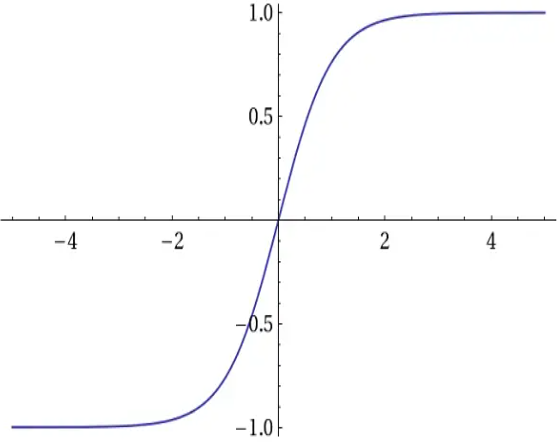
\includegraphics[width=2.2in]{./figures/tanhcurve.png}
                \caption{ Tanh curve}
            \end{figure} \\
            \item {\bf ReLU:} ReLU stands for Rectified Linear Unit. Although it gives an impression of a linear function, ReLU has a derivative function and allows for backpropagation while simultaneously making it computationally efficient. The main catch is that ReLU function does not activate all the neurons at the same time. The neurons will only be deactivated if the input to the ReLU function is less than zero.
            \begin{figure}[ht]
                \centering
                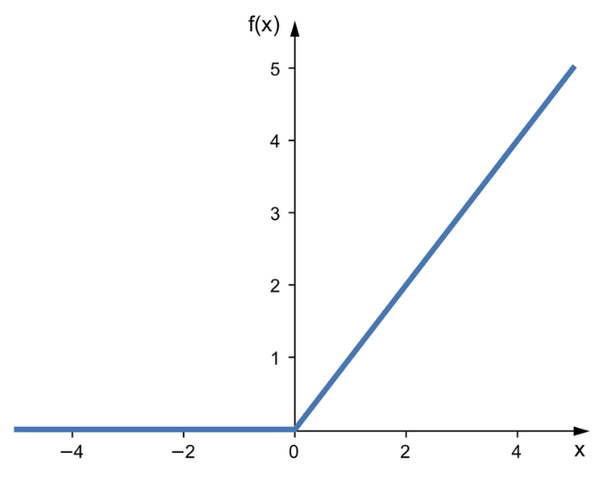
\includegraphics[width=2.5in]{./figures/relucurve.png}
                \caption{ Relu curve}
            \end{figure} \\
            Mathematically it can be represented as:
            $$R(x) =\left \{\frac{x}{0} \ \ \ \ \begin{matrix}
                if \ x\geq 0 & \\ if \ x < 0
                & 
               \end{matrix} \right\}$$
               The major limitation of ReLU is Dying ReLU problem. The negative side of the graph makes the gradient value zero. Due to this reason, during the backpropagation process, the weights and biases for some neurons are not updated. This can create dead neuron which never get activated.
            \item {\bf Leaky Relu:} : Leaky ReLU is an improved version of ReLU function to solve the Dying ReLU  problem as it has small positive slope in the negative area. The advantage of Leaky ReLU is same as ReLU, in addition to the fact that it does enable backpropagation, even for negative input values. By making this minor modification for negative input values, the gradient of the left side of the graph comes out to be a non-zero value.\\
            The limitation faced by Leaky ReLU is the prediction may not be consistent for negative input values.\\
            Mathematically it can be represented as:
            $$f(x) =\left \{\frac{x}{0} \ \ \ \ \begin{matrix}
                if \ x\geq 0 & \\ if \ \alpha * x < 0
                & 
               \end{matrix} \right\}$$
            \begin{figure}[ht]
                \centering
                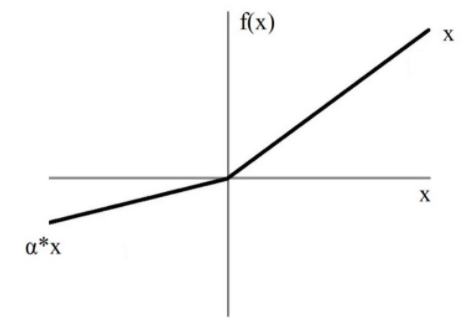
\includegraphics[width=2.6in]{./figures/leakyrelucurve.png}
                \caption{Leaky Relu curve}
            \end{figure}
            \item {\bf Prelu:}Parametric ReLU is another variant of ReLU that aims to solve the problem of gradient’s becoming zero for the left half axis. This function provides the slope of the negative part of the function as an argument. 
            \begin{figure}[ht]
                \centering
                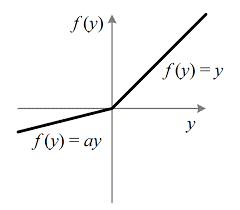
\includegraphics[width=2.5in]{./figures/prelucurve.png}
                \caption{Parametric Relu curve}
            \end{figure} \\
            Mathematically it can be represented as:
            $$R(x) =\left \{\frac{x}{0} \ \ \ \ \begin{matrix}
                if \ x\geq 0 & \\ if \ a * x < 0
                & 
               \end{matrix} \right\}$$
               where ‘a’ is the slope parameter for negative values. Prelu can learn slope parameter using backpropagation at a negligible increase in the cost of training.
        \end{itemize}
        \item {\bf Pixel Shuffle:} The Pixel shuffle is a technique used in image super resolution to upscale an image by a factor of r. It works by rearranging the pixels in a feature map of size $(W,H,C * r^2)$ to form a super-pixel feature map of size (r*W, r*H, C).\\The pixel shuffle operation can be described as follows:
        \begin{itemize}
            \item For each pixel in the input feature map, split its value into $r^2$ sub-pixels.
            \item Arrange the sub-pixels in grid-like pattern, with each sub-pixels occupying a position in a feature map
        \end{itemize}
        \begin{figure}[ht]
            \centering
            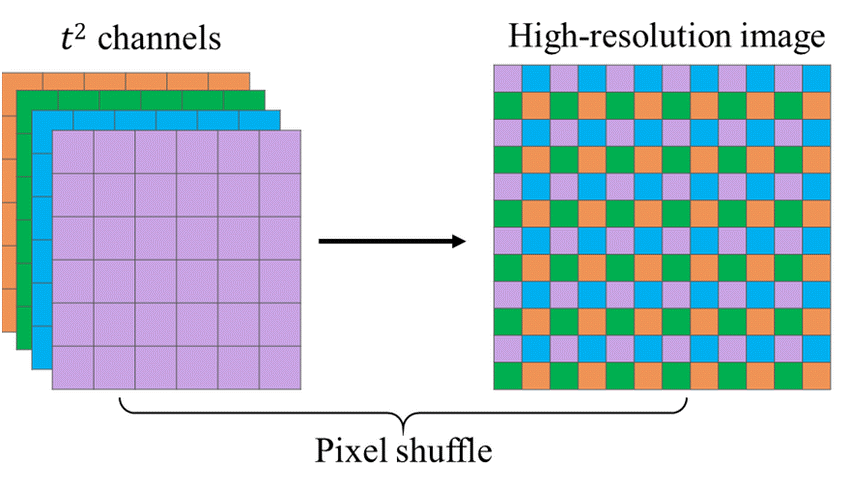
\includegraphics[width=3in]{./figures/pixelshuffle.png}
            \caption{Pixel Shuffle}
        \end{figure}
        \item {\bf Residual Block:} A residual block is a building block that contains one or more convolutional layers and a skip connection. The skip connection allows gradient to flow through the network more efficiently, improving the training process and avoiding the vanishing gradient problem.
        \begin{figure}[h!]
            \centering
            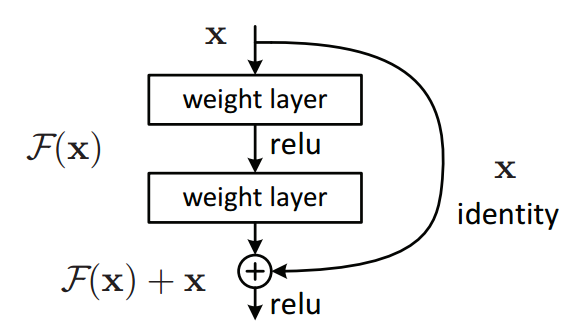
\includegraphics[width=3in]{./figures/residualblock.png}
            \caption{Residual block}
        \end{figure}
    \end{enumerate}


\newpage
\section{METHODOLOGY}
Image Super Resolution is a branch of Artificial Intelligence that deals with upscaling a Low-Resolution Image to High Resolution Image, filling in the missing pixels with the different techniques.

% \newpage
\section{FEASIBLITY ANALYSIS}
We are planning to use deep learning to develop a system that can increase the
resolution of image. The system is trained on dataset of high-resolution images and
low-resolution images generated using degradation model to generate high resolution
images from low resolution images.\\
Deep learning is shown to be very effective for ISR. There are many models
developed for this task we can take inspiration from. The technical feasibility of this
project is therefore high. The cost of developing the system will depend on the size of
the dataset used to train the model, and the complexity of the model. As we are planning
to train the model on server and deploy the system on cloud-based service. So, server
costs will be our main cost for this project. \\
The technical and economic feasibility analysis show that we can complete this
project successfully.
\newpage
\section{RESULT AND DISCUSSION}
\subsection{Work Completed:}
As we are planning on comparison of different methods. We have selecteed few methods like SRCNN, SRGAN, and ESRGAN. SRGAN involves residual network SRResNet which will be also used as baseline for SRGAN. We have trained and tested SRGAN on various sets of data involving CelebA, DIV2k, Flickr2k, OST and COCO(2014). CoCo has a large and diverse set of data and it perfromed well thats why we are finalizing this dataset for training further methods. 
\subsection{Work Remaining}
\begin{enumerate}
    \item We have not trained models for SRCNN and ESRGAN yet.
    \item We don't have a polished website to showcase our results.
\end{enumerate}  
\subsection{Limitations}
Few limitations related to SRGAN that we have trained are:
\begin{enumerate}
    \item The implementation and training of SRGAN demand substantial computational resources, posing challenges in terms of the time and hardware needed.
    \item  The effectiveness of SRGAN relies heavily on the availability of a sizable and diverse training dataset, presenting challenges in obtaining and curating such data.
    \item There is alot of subjectivity in evaluating the images as quantative metrics can't identify human perception.
    \item  The study lacks comparison with real-world benchmarks or scenarios.
    \item Due to constraints, we couln't explore tinkering hyperparameters.
    \item The study lacks a direct comparison with the latest state-of-the-art super-resolution techniques.
\end{enumerate}
% \subsection{Problem Faced}
% \subsection{Budget Analysis}
\subsection{Work Schedule:}
\newcolumntype{P}[1]{>{\raggedright\vrule height4ex width 0pt}p{#1}<{\vrule depth 2.5ex width 0pt}}
    \begin{tabular}{|P{6cm}*{10}{|c}|}
    \hline
    \centering \raisebox{-2ex}[0pt][0pt]{Action plan} & \multicolumn{7}{c|}{2023} & \multicolumn{3}{c|}{2024} \\
    \cline{2-11}
    \multicolumn{1}{|c|}{\vphantom{$\Big|$}} &
    \scriptsize Jun & \scriptsize Jul & \scriptsize Aug & \scriptsize Sep &
    \scriptsize Oct & \scriptsize Nov & \scriptsize Dec & \scriptsize Jan &
    \scriptsize Feb & \scriptsize Mar \\
    \hline
    Research &
    {\cellcolor{gray}} &{\cellcolor{gray}}&{\cellcolor{gray}}&{\cellcolor{gray}}&{\cellcolor{gray}}&&&&& \\
    \hline
    Data Acquisition &
    && {\cellcolor{gray}} &{\cellcolor{gray}} &{\cellcolor{gray}} &&&&& \\
    \hline
    Model Development and Evaluation &
    &&&&{\cellcolor{gray}} &{\cellcolor{gray}}&{\cellcolor{gray}}&&& \\
    \hline
    Model Deployment &
    &&&&&&{\cellcolor{gray}}&{\cellcolor{gray}}&{\cellcolor{gray}} & \\
    \hline
    Prepare the report and presentation &
    &&&&&&{\cellcolor{gray}}&{\cellcolor{gray}}&{\cellcolor{gray}}&{\cellcolor{gray}} \\
    \hline
    \end{tabular}
%\bibliographystyle{apalike}
\newpage
\bibliographystyle{IEEEtran}
\bibliography{sections/references.bib}
% \newpage
\section{Appendix}
\subsection{Work Schedule:}
\newcolumntype{P}[1]{>{\raggedright\vrule height4ex width 0pt}p{#1}<{\vrule depth 2.5ex width 0pt}}
    \begin{tabular}{|P{6cm}*{10}{|c}|}
    \hline
    \centering \raisebox{-2ex}[0pt][0pt]{Action plan} & \multicolumn{7}{c|}{2023} & \multicolumn{3}{c|}{2024} \\
    \cline{2-11}
    \multicolumn{1}{|c|}{\vphantom{$\Big|$}} &
    \scriptsize Jun & \scriptsize Jul & \scriptsize Aug & \scriptsize Sep &
    \scriptsize Oct & \scriptsize Nov & \scriptsize Dec & \scriptsize Jan &
    \scriptsize Feb & \scriptsize Mar \\
    \hline
    Research &
    {\cellcolor{gray}} &{\cellcolor{gray}}&{\cellcolor{gray}}&{\cellcolor{gray}}&{\cellcolor{gray}}&&&&& \\
    \hline
    Data Acquisition &
    && {\cellcolor{gray}} &{\cellcolor{gray}} &{\cellcolor{gray}} &&&&& \\
    \hline
    Model Development and Evaluation &
    &&&&{\cellcolor{gray}} &{\cellcolor{gray}}&{\cellcolor{gray}}&&& \\
    \hline
    Model Deployment &
    &&&&&&{\cellcolor{gray}}&{\cellcolor{gray}}&{\cellcolor{gray}} & \\
    \hline
    Prepare the report and presentation &
    &&&&&&{\cellcolor{gray}}&{\cellcolor{gray}}&{\cellcolor{gray}}&{\cellcolor{gray}} \\
    \hline
    \end{tabular}

\end{document}